\section{Experimental Results}

\subsection{Experimental setup}

The experiments are conducted on antibiotic-specific datasets prepared from the same shared genotype-phenotype cohort. The same cohort selection rules, phenotype cleaning rules, and genotype normalization rules are applied across all scopes to keep the comparison fair. The current implementation evaluates 14 antibiotics that satisfy the minimum sample and class-count thresholds required for stable supervised learning.

The main model-based comparison includes three determinant-connection scopes:

\begin{itemize}
    \item \textbf{Strict ML}
    \item \textbf{Broad ML}
    \item \textbf{All ML}
\end{itemize}

The direct genotype-to-phenotype baseline is implemented in two forms:

\begin{itemize}
    \item \textbf{Strict rule-based}
    \item \textbf{Broad rule-based}
\end{itemize}

This comparison is more meaningful for this bioinformatics study than comparing several generic classifiers because it isolates the effect of biological scope and prior knowledge.

\subsection{Average performance across methods}

Table~\ref{tab:method-average-metrics} summarizes the average performance of the five main method settings across the 14 antibiotics.

\begin{table}[H]
\centering
\caption{Average performance across antibiotics}
\label{tab:method-average-metrics}
\small
\begin{tabular}{lccccc}
\toprule
Method & Accuracy & Precision & Recall & ROC-AUC & Avg. zero rows \\
\midrule
Strict rule-based & 0.861 & 0.655 & 0.704 & -- & 4461.1 \\
Broad rule-based  & 0.839 & 0.648 & 0.987 & -- & 3790.5 \\
Strict ML         & 0.822 & 0.744 & 0.865 & 0.842 & 4461.1 \\
Broad ML          & 0.988 & 0.972 & 0.974 & 0.984 & 3790.5 \\
All ML            & 0.987 & 0.966 & 0.974 & 0.988 & 0.0 \\
\bottomrule
\end{tabular}
\end{table}

Several patterns are immediately visible. First, \textit{broad ML} and \textit{all ML} are the strongest overall settings, both achieving average accuracy near 0.99 and average recall around 0.974. Second, \textit{broad rule-based} has the highest average recall among the direct rule methods, reaching 0.987, but this comes with a clear loss in precision and specificity. Third, the \textit{strict} settings use a narrower biological scope but suffer from many zero-hit or zero-feature rows, especially for some beta-lactam antibiotics.

\subsection{Observed performance pattern of the ML scopes}

The model-based results show a clear overall pattern. The \textit{all} scope gives the best ability to separate resistant and susceptible isolates across antibiotics and removes the zero-feature problem completely. Its average ROC-AUC is 0.988, higher than the 0.984 achieved by \textit{broad ML} and much higher than the 0.842 of \textit{strict ML}. The \textit{broad} scope performs competitively for many antibiotics and is the strongest constrained alternative. The \textit{strict} scope is still useful as a narrow reference, but it is too fragile to serve as the default setting because it leaves too many isolates with no usable determinant evidence.

\begin{figure}[H]
\centering
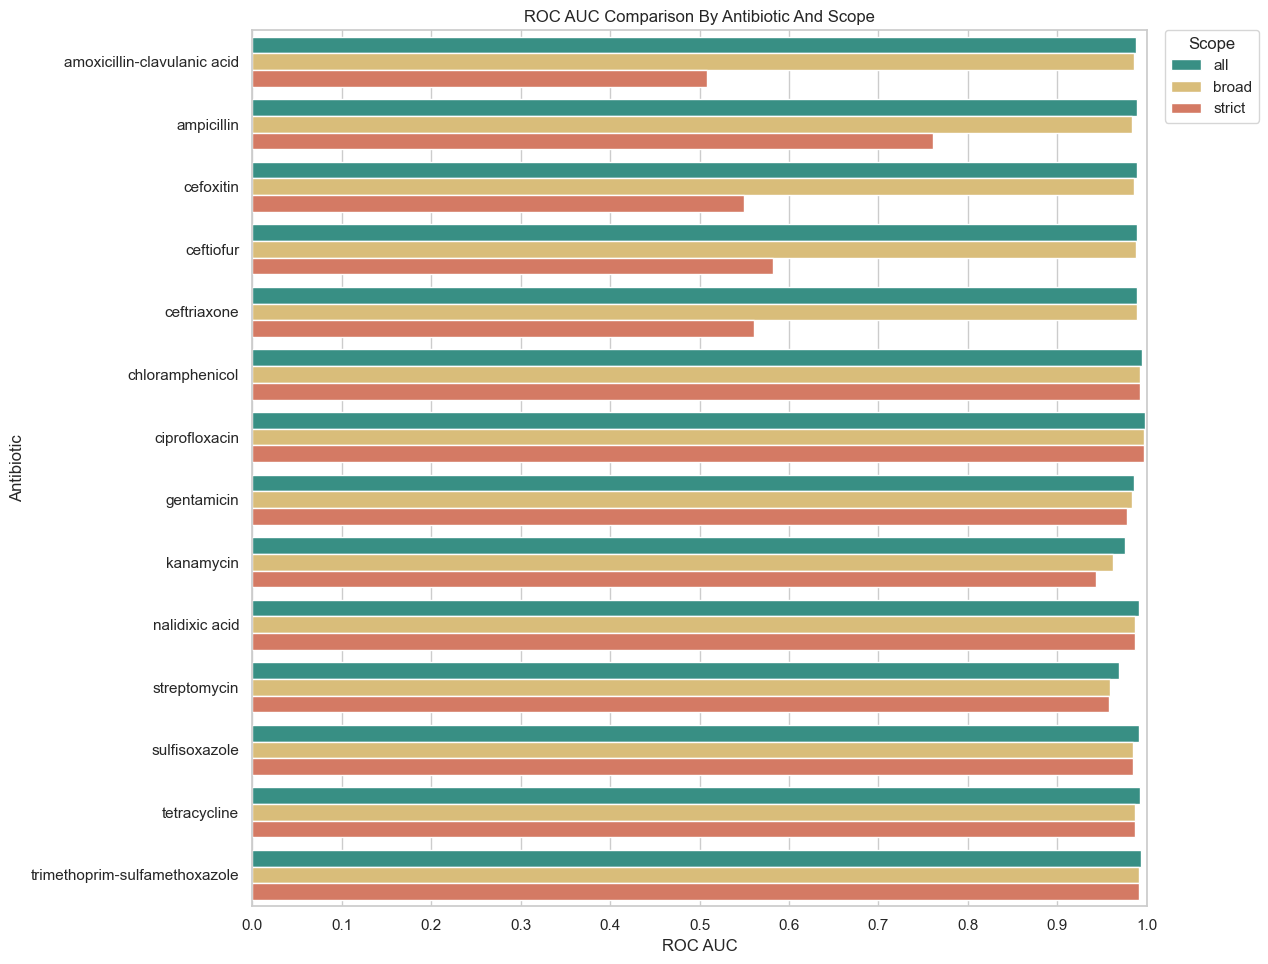
\includegraphics[width=0.95\textwidth]{figures/roc_auc_by_scope}
\caption{ROC-AUC comparison across antibiotics and determinant-connection scopes.}
\label{fig:roc-auc-by-scope}
\end{figure}

This pattern is biologically interpretable. Narrow matching improves feature specificity, but it can also exclude genes or mutations that are still useful within the same broader drug family. Relaxing the scope to \textit{broad} captures more same-class mechanisms, while the \textit{all} setting allows the model to use wider patterns among many detected determinants.

\subsection{Main result trends}

The results support four main conclusions:

\begin{enumerate}[label=\arabic*.]
    \item The \textit{all} scope is the strongest global default when the main objective is predictive performance.
    \item The \textit{broad} scope is the best compromise when interpretability is still important.
    \item The \textit{strict} scope is useful as a narrow biological baseline, but it fails on several antibiotics because the matching rule is too restrictive.
    \item Performance differences across antibiotics reflect real differences in resistance mechanism diversity and determinant coverage.
\end{enumerate}

\subsection{Rule-based versus machine-learning behavior}

The rule-based baselines are useful because they show when the presence of known determinants is already enough to predict phenotype and when machine learning adds real value. For some antibiotics, the direct rule is already very strong. For example, under the strict scope, ciprofloxacin reaches precision 0.968 and recall 0.998, chloramphenicol reaches precision 0.990 and recall 0.988, and nalidixic acid reaches precision 0.953 and recall 0.989. These results suggest that, for such antibiotics, the detected genes and mutations already match the phenotype closely.

However, the same direct rule becomes too weak or too coarse for other antibiotics. Under the strict rule baseline, ceftriaxone reaches recall only 0.101 and precision 0.090, while ceftiofur reaches recall 0.133 and precision 0.102. When the scope is relaxed to broad rule-based inference, recall for ceftriaxone increases sharply to 0.985, but precision remains only 0.489. This shows the main trade-off clearly: broader matching can recover missed resistant isolates, but it can also overcall resistance by accepting determinants that are related to the same drug class but are not specific enough to the target drug.

Machine learning changes this balance substantially. For ceftriaxone, \textit{broad ML} achieves precision 0.992 and recall 0.976, while \textit{all ML} achieves precision 0.990 and recall 0.974. In other words, the learned models keep the broad coverage needed to recover resistant isolates, but avoid much of the precision loss seen in broad rule-based inference. A similar pattern appears for ceftiofur and cefoxitin. These comparisons support the main scientific argument of the report: machine learning is most valuable when broader determinant evidence must be combined more carefully than a direct rule can do.

\subsection{Interpretation of zero-hit and zero-feature rows}

One of the clearest signals in the experiment is the role of zero rows. In the rule-based setting, a zero-hit row means that no determinant connected to the target antibiotic scope was found in the isolate. In the machine-learning setting, the corresponding zero-feature row means the model received an all-zero feature vector for that isolate. The averages in Table~\ref{tab:method-average-metrics} show that both strict settings suffer from roughly 4461 zero rows on average, whereas broad settings reduce this burden to about 3790 rows, and the all scope removes it entirely.

This result explains much of the performance gap between strict and broader settings. A narrow scope can be biologically conservative, but if it leaves too many isolates without usable determinant evidence, both rule-based prediction and machine learning start from a weak input.

\subsection{Discussion of limitations}

The current study predicts a binary resistant/susceptible phenotype rather than MIC, uses curated determinant resources rather than full pan-genome features, and has not yet performed external validation on an independent surveillance cohort. These limitations do not invalidate the study, but they define its scope clearly and position it as a determinant-based bioinformatics analysis rather than a full clinical deployment study.
